\section{Experiment 1}
In this experiment we would like to perform validation on our solution of $\phi$ as to see if we get the expected results. First we will investigate how we expect our solution to look like. From \cite{wiki} we have the illustrations in \autoref{wiki}. In \autoref{wiki1} and \autoref{wiki2} we have a close up view of the electric field around a positive and negative point charge. Where here see the contour lines around the centers are circular and that the electric field lines are perpendicular to these contours. In \autoref{wiki2} we again see the two charges, but now opposite each other. We see that the contours drawn gets effected by the other charge, and had there been drawn more contours we would have seen they would get prolonged as they got closer to the middleground. We also see the full size of the electric field lines. This is what we will expect to see from our model.\\
We can now compute our solution for $\phi$ on different grid sizes and resolutions and visually validate our model. In \autoref{results} we see our results of this. We note that the white lines have been manually drawn to give an idea of how the electrical field lines would look like. These have been attempted drawn such that they are perpendicular to the contour lines, as they represent the direction of $\nabla\phi$. 

\begin{figure}
	\centering
	\begin{subfigure}[b]{\linewidth}
		\centering
		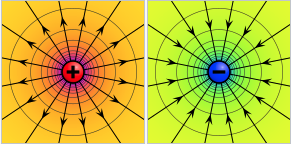
\includegraphics[width=\linewidth]{Materials/wiki1}
		\caption{Electric potential of seperate positive and negative point charges.}
		\label{wiki1}
	\end{subfigure}
	\\
	\begin{subfigure}[b]{0.7\linewidth}
		\centering
		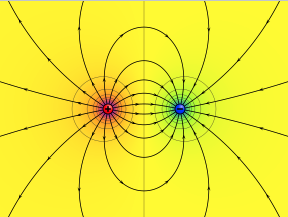
\includegraphics[width=\linewidth]{Materials/wiki2}
		\caption{Electric potential near two opposite point charges.}
		\label{wiki2}
	\end{subfigure}
	\caption{Illustrations of electric potential.}
	\label{wiki}
\end{figure}

\begin{figure}
	\centering
	\begin{subfigure}[b]{0.49\linewidth}
		\centering
		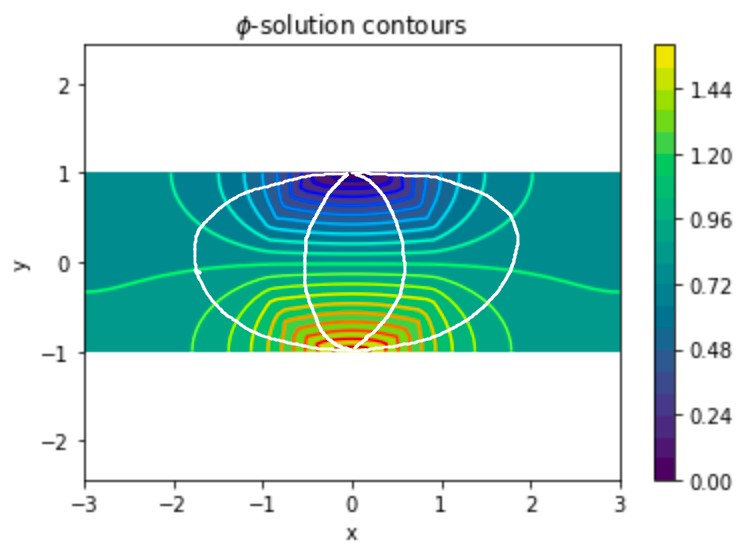
\includegraphics[width=\linewidth]{Materials/627224}
		\caption{Grid size: 6 by 2, resolution: 72 by 24.}
	\end{subfigure}
	\hfill
	\begin{subfigure}[b]{0.49\linewidth}
		\centering
		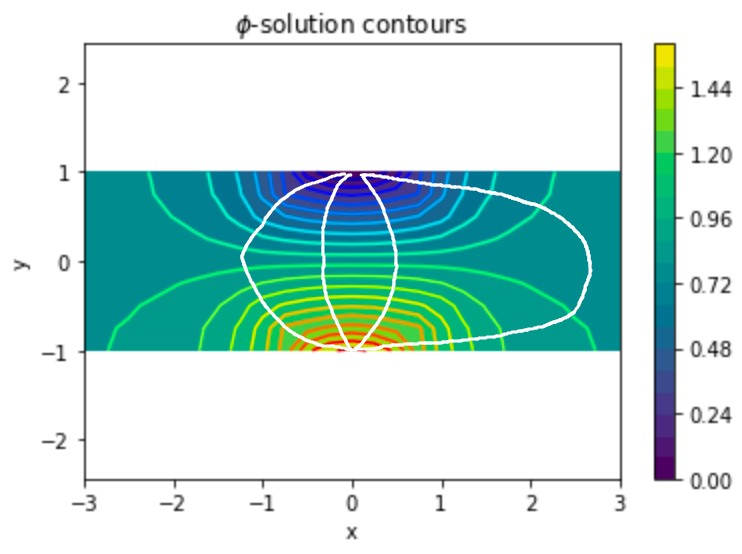
\includegraphics[width=\linewidth]{Materials/62248}
		\caption{Grid size: 6 by 2, resolution: 24 by 8.}
	\end{subfigure}
	\\
	\begin{subfigure}[b]{0.49\linewidth}
		\centering
		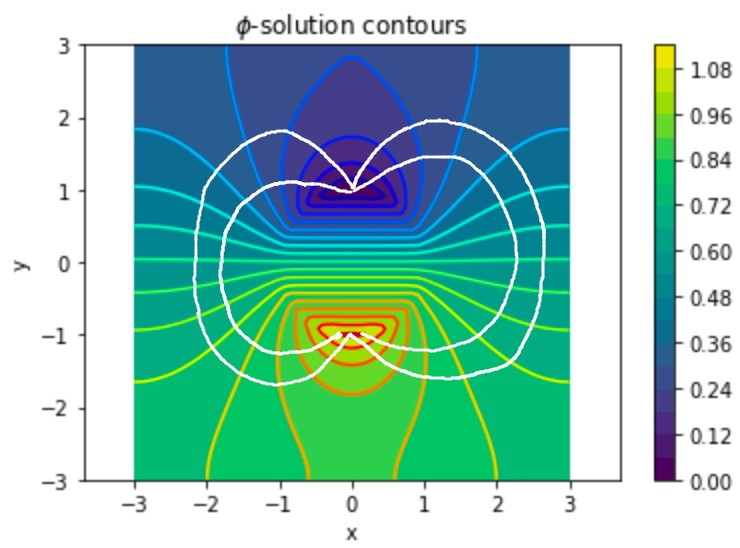
\includegraphics[width=\linewidth]{Materials/667272}
		\caption{Grid size: 6 by 6, resolution: 72 by 72.}
	\end{subfigure}
	\hfill
	\begin{subfigure}[b]{0.49\linewidth}
		\centering
		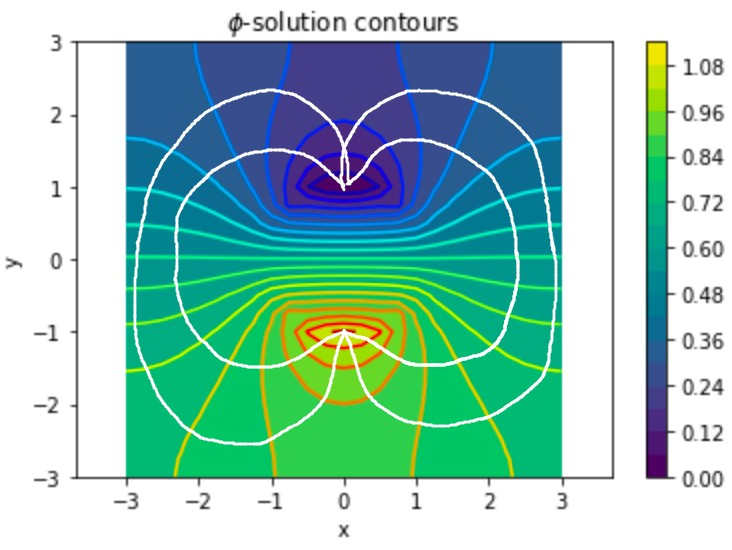
\includegraphics[width=\linewidth]{Materials/662424}
		\caption{Grid size: 6 by 6, resolution: 24 by 24.}
	\end{subfigure}
	\caption{Results for solving the potential field $\phi$ for different grid sizes and resolution.}
	\label{results}
\end{figure}

\subsection{Discussion of results}
The first thing we note about our results is all contour lines are rather 'square' and not as perfect round as we had expected. This is probably due to error introduced when we handle the unit circle, but can perhaps also partially stem from the error introduced due to the boundary conditions. We do see however, that as we move towards the middle of the poles, the contours correctly get flat and prolonged. We also note on the 6 by 6 grids that the contours are round behind the poles, more so on the finer resolution image than the coarse. When we look at the electrical field lines in white, we see the lines behaves as expected, going in an arc from one pole to the other. In conclusion we do have some errors, probably due to the handling of the unit circle discretization, but in broad lines, our model is in accordance to our expectation.